%
%  untitled
%
%  Created by Johan Boissard [] on 2010-06-24.
%  Copyright (c) Johan Boissard. All rights reserved.
% hhh

\documentclass[a4paper,titlepage] {scrartcl}
\usepackage[T1]{fontenc}
\usepackage[utf8]{inputenc}
\usepackage{graphicx}
\usepackage{engord}
%\usepackage[english]{babel}
\usepackage{fancyhdr}
\usepackage{amsmath}
\usepackage{comment}

\usepackage{listings}

%allows inclusion of url (hyperref is better than url) 
%ref: http://www.fauskes.net/nb/latextips/
\usepackage{hyperref}

%package for chemistry ie: \ce{(NH4)2SO4 -> NH4+ + 2SO4^2-} 
%ref:www.ctan.org/tex-archive/macros/latex/contrib/mhchem/mhchem.pdf
\usepackage[version=3]{mhchem}
%celsius + degrees
\usepackage{gensymb}
%to get last page
\usepackage{lastpage} % \pageref{LastPage}

%make use of the fullpage (no HUGE margins)
\usepackage{fullpage}
\usepackage{subfig}

%allows separating cell in table by diagonal line
\usepackage{slashbox}




%\renewcommand{\chaptername}{Laboratory}
%\setcounter{chapter}{5}

\usepackage{color}
\usepackage[usenames,dvipsnames, table]{xcolor}
% Include this somewhere in your document



\usepackage[absolute]{textpos}

%column  of multi row in tables
\usepackage{multirow}

%to have vertical text in table
\usepackage{rotating}


%%%%%%% a virer ici!!!!
\begin{comment}
%Fonts and Tweaks for XeLaTeX
\usepackage{fontspec,xltxtra,xunicode}
%\defaultfontfeatures{Mapping=tex-text}
%\setromanfont[Mapping=tex-text]{Hoefler Text}
\setsansfont[Scale=MatchLowercase,Mapping=tex-text]{Gill Sans}

\definecolor{shade}{HTML}{D4D7FE}	%light blue shade
\definecolor{text1}{HTML}{272727}		%text is almost black
\definecolor{headings}{HTML}{173849} 	%dark blue %%%dark red 70111
\definecolor{title}{HTML}{173849} 	%dark blue %%%dark red 70111

\usepackage{titlesec}				%custom \section
\end{comment}







\author{Johan Boissard}
\date{\today}
\title{$\mu$-Economics}
\begin {document}

\maketitle
%\tableofcontents

\section{Introduction to Economics}
\subsubsection{Economy} "the one who manages a household", in greek. Economics is the study of how sociey manages its scarce resources.

\subsubsection{Scarcity}
means that society has limited resources and therefore cannot produce all the goods and service people wish to have.

\subsection{Ten principles of Economics}
\begin{comment}
\subsubsection{People Face Trade-Offs}
\subsubsection{The cost of Something is what you give up to get it}
\subsubsection{Rational People Think at the Margin}
\subsubsection{People respond to Incentives}
\subsubsection{Trade can make everyone better off}
\subsubsection{Markets are usually a good way to organize Economic Activity}
\subsubsection{Governments can sometimes improve Market Outcome}
\subsubsection{An Economy's Standard of Living depends on its ability to produce Goods and Services}

\subsubsection{Prices rise when the governments prints too much Money}
\subsubsection{Society faces a short-run Trade-off between Inflation and Unemployment}
\end{comment}
\begin{enumerate}
	\item People Face Trade-Offs: there is no such things as a free lunch
	\item The cost of Something is what you give up to get it: decisions require comparing costs and beefits of alternatives
	\item Rational People Think at the Margin: marginal changes are small, incrmental adjustements to an existing plan of action: People make decisions by comparing 
	costs and benefits at the margin.
	\item People respond to Incentives
	\item Trade can make everyone better off
	\item Markets are usually a good way to organize Economic Activity
	\item Governments can sometimes improve Market Outcome
	\item An Economy's Standard of Living depends on its ability to produce Goods and Services
	\item Prices rise when the governments prints too much Money
	\item Society faces a short-run Trade-off between Inflation and Unemployment
\end{enumerate}

\subsection{Economic Models}
\subsubsection{The Circular flow diagram}
The circular flow model is a visual model that shows ahow dollars and goods flow through markets among households and firms.
\subsubsection{The production possibility frontier}
This model is a graph that shows the combination of output that the economy can produce given the available factors of production and the available production technology.

\subsection{Opportunity Cost}
In a two-goods economy: the amount of good A you have to forego in order to get a certain amount of a special good B represents the \textbf{opportunity cost} of product B.

\subsection{Real vs nominal price}
\label{sub:realVsNominal}
\subsubsection{Nominal Price}
Absolute pric of a good; unadjusted for inflation
\subsubsection{Real Price}
Price of a good relative to an aggregate measure of prices; price adjusted for inflation

\subsection{Macro- vs Microeconomics}
\subsubsection{Micro}
Focuses on the individual parts of the economy
\subsubsection{Macro}
looks at the economy as a whole

\subsection{Normative and Positive Economics}
\subsubsection{Normative}
deals with ethical questions ? (bullshit)
\subsubsection{Positive}
describe the facts of an economy and its behavior


%lecture 2
\section{Supply and Demand: How Markets work}
\subsection{Market}
The market is a collection of buyers and sellers, that through their actual or potential interactions determine the price of a product or set of products. 

\subsubsection{Competitive Market}
market in which there are many buyers and sellers so that each ha s a negligible impact on the price.

Buyers and sellers are \textbf{price takers}.

\subsubsection{Other market forms}
\begin{enumerate}
	\item Monopoly: one seller that control the price
	\item Oligopoly: few sellers
	\item Monopolistic Competition: many sellers, slightly differentiated products (e.g. magazines), each seller may set price for its own product
\end{enumerate}

\subsection{Supply and Demand}
are the force that make the market economy work. They determine the quantity the quantity of each good to be produced and the price at which it is sold. Economists use the model of supply and demand to analyze competitive markets.

\subsubsection{Demand}
Law of demand states that quantity of good demanded falls when its price rises
\begin{eqnarray*}
	\frac{dQ_d}{dP}\leq0
\end{eqnarray*}

\subsubsection{Supply}
law of supply states that the quantity of goods supplied rises when price rises.
\begin{eqnarray*}
	\frac{dQ_s}{dP}\geq0
\end{eqnarray*}
\subsubsection{Equilibrium Price}
where the supply curve equals the demand curve
\begin{eqnarray*}
	Q_d(P^*)=Q_s(P^*)
\end{eqnarray*}
where $P^*$ is the optimal price.

\subsubsection{Surplus or excess supply}
\begin{figure}[htbp]
	\centering
		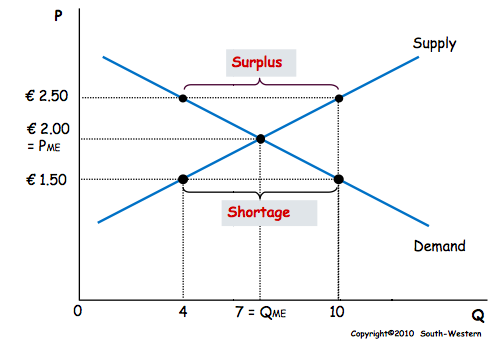
\includegraphics[height=3in]{images/surplusshortage.png}
	\caption{Surplus and shortage}
	\label{fig:images_surplusshortage}
\end{figure}

\begin{eqnarray*}
	P>P^* \Rightarrow Q_s >Q_d 
\end{eqnarray*}
Suppliers will lower the price to increase sales, thereby moving toward equilibrium. 
\subsubsection{Shortage or excess demand}
\begin{eqnarray*}
	P<P^* \Rightarrow Q_d > Q_s
\end{eqnarray*}
Suppliers will raise the price due to too many buyers chasing too few goods.

\subsection{Elasticity}
is a measure of how much buyers and sellers respond to changes in market conditions

\subsubsection{Price elasticity of demand}
\begin{eqnarray*}
	E_d=\frac{\text{\% change in quantity}}{\text{\% change in price}}=
	\frac{dQ_d}{dP}\frac{P}{Q_d}
\end{eqnarray*}
Total revenue: $TR = P \cdot Q$


\begin{eqnarray*}
	\text{Income elasticity of demand} = 
	\frac{\text{\% change in quantity demanded}}{\text{\% change in income}}
\end{eqnarray*}

\begin{eqnarray*}
	\text{Cross-price elasticity of demand} = 
	\frac{\text{\% change in quantity demanded of good 1}}{\text{\% change in the price of good 2}}
\end{eqnarray*}

\begin{eqnarray*}
	\text{Price elasticity of supply} = 
	\frac{\text{\% change in quantity supplied}}{\text{\% change in price}}
\end{eqnarray*}

\subsection{Behavioral Economics}
\begin{itemize}
	\item People as well as their decisions aren't always rational!
	\item People do care about fairness (at least some ...)
\end{itemize}

%lecture 3


\begin{comment}
%\chapter{Strategic Supply Chain Management}
%lecture 1
\section{Supply chain entities and processes}
%lecture 2
\section{Strategic fit between supply chain and competitive strategy}

A supply chain includes R\& D engineering, marketing and sales, operations (logistics, manufacturing, assembly), purchasing and supply, finance, customer service.
\end{comment}

\section{Supply, Demand and Government Policies}
\subsection{Estimation of demand curve}
Using empirical data and then \textbf{regression}

\subsection{Controls o prices}
\begin{itemize}
	\item Price ceiling
	\item Price Floor
\end{itemize}

\paragraph{Price Ceiling} % (fold)
If price is set above equilibrium: \textbf{not binding}, otherwise \textbf{binding}
\label{par:price_ceiling}
\begin{figure}[htbp]
	\centering
		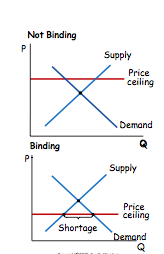
\includegraphics[height=3in]{images/ceiling.png}
	\caption{Price ceiling}
	\label{fig:images_ceiling}
\end{figure}

% paragraph price_ceiling (end)

\paragraph{Price floor} % (fold)
If price floor is set above the equilibrium: \textbf{binding}, otherwise \textbf{not binding}.
\label{par:price_floor}
\begin{figure}[htbp]
	\centering
		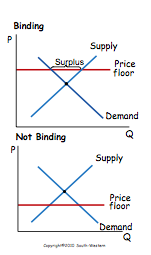
\includegraphics[height=3in]{images/floor.png}
	\caption{Price floor}
	\label{fig:images_floor}
\end{figure}

% paragraph price_floor (end)

\subsection{Taxes}
\paragraph{Taxes on Buyers} % (fold)
\label{par:taxes_on_buyers}

% paragraph taxes_on_buyers (end)
\begin{figure}[htbp]
	\centering
		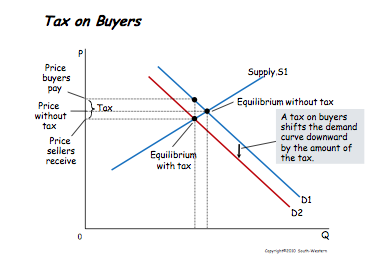
\includegraphics[height=3in]{images/taxBuyers.png}
	\caption{Tax on Buyers}
	\label{fig:images_taxBuyers}
\end{figure}

\paragraph{Taxes on sellers} % (fold)
\label{par:paragraph_name}

\begin{figure}[htbp]
	\centering
		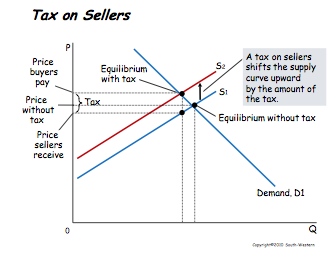
\includegraphics[height=3in]{images/taxSellers.png}
	\caption{Tax on Sellers}
	\label{fig:images_taxSellers}
\end{figure}

\paragraph{Elasticity and Tax Incidence} % (fold)
\label{par:elasticity_and_tax_incidence}
Depending on the elasticity of the demand and/or supply the burden of the tax is shared inequally.
% paragraph elasticity_and_tax_incidence (end)

\section{Welfare Economics and Deadweight Loss}

\subsection{Welfare Economics}
Do the equilibrium price and quantity of the allocated 
scarce resources maximize the total welfare of buyers 
and sellers?

Welfare economics is the study of how the allocation 
of resources affects economic well-being.

\subsection{Consumer surplus ($CS$)}
\begin{figure}[htbp]
	The total area below the demand curve and above the price is the 
	sum of the consumer surplus of all buyers in the market for a good or 
	service. 
	
	\begin{equation}
		CS=\int_{P^*}^{P_{\text{max}}}Q_D(P)dP
	\end{equation}

	\centering
		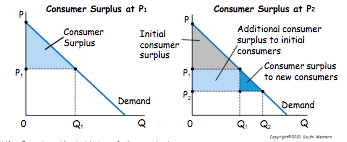
\includegraphics[height=2in]{images/consumer surplus.png}
	\caption{Consumer surplus}
	\label{fig:images_consumer surplus}
\end{figure}

\subsection{Producer Surplus ($PS$)}
Measures economic welfare from the producer's side

\begin{equation}
	PS=\int_{P_{\text{min}}}^{P^*}Q_S(P)dP
\end{equation}

\begin{figure}[htbp]
	\centering
		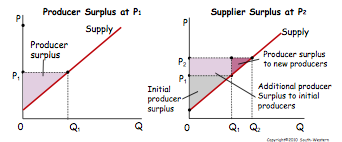
\includegraphics[height=2in]{images/prodSurplus.png}
	\caption{Producer's surplus}
	\label{fig:images_prodSurplus}
\end{figure}


\subsection{Total Surplus}
\begin{eqnarray*}
	\text{Total surplus} &=&  \text{Consumer surplus} + \text{Producer surplus}\nonumber\\
	&=& \text{Value to buyers} + \text{Cost to sellers}
\end{eqnarray*}

\subsection{Market Efficiency}
\paragraph{Benevolent Social Planner (BSP)} % (fold)
\label{par:benevolent_social_planner_bsp_}
wants to maximize the economics well-being of everyone in society
% paragraph benevolent_social_planner_bsp_ (end)

\begin{enumerate}
	\item \textbf{Efficiency}: the property of a resource allocation of maximizing the total surplus received by all members of the society
	\item \textbf{Equity}: the fairness of the distribution of well-being among the buyers and sellers.
	
	
\end{enumerate}
\begin{figure}[htbp]
	\centering
		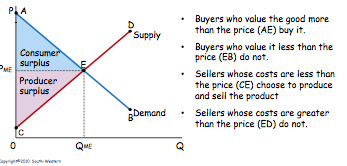
\includegraphics[height=2in]{images/mrktEff.png}
	\caption{Market Efficiency}
	\label{fig:images_mrktEff}
\end{figure}

\begin{enumerate}
	\item BSP should not alter market outcome
	\item Byers and sellers are guided by an \textbf{invisible hand} (Adam Smith)
\end{enumerate}

\subsection{Deadweight Loss of Taxation} % (fold)
\label{sub:deadweight_loss_of_taxation}
\begin{eqnarray*}
	\text{Tax Revenue} = \underbrace{T}_{\text{Size of the tax}} 
						\cdot 
						\overbrace{Q}^{\text{Quantity of goods sold}} 
\end{eqnarray*}
% subsection deadweight_loss_of_taxation (end)
%%%%%%%%

\paragraph{Tax Revenues} % (fold)
\label{par:tax_revenues}
\begin{figure}[htbp]
	\centering
		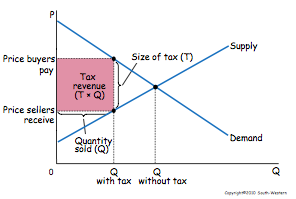
\includegraphics[height=3in]{images/taxRev.png}
	\caption{Tax Revenues}
	\label{fig:images_taxRev}
\end{figure}

% paragraph tax_revenues (end)

\paragraph{Deadweight Loss} % (fold)
\label{par:deadweight_loss}
\begin{figure}[htbp]
	\centering
		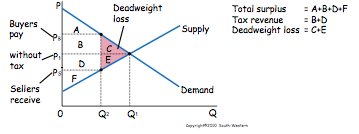
\includegraphics[height=2in]{images/deadweightLoss.png}
	\caption{Deadweight Loss}
	\label{fig:images_deadweightLoss}
\end{figure}

% paragraph deadweight_loss (end)



\section{International Trade}
\label{sec:international_trade}
\subsection{Interdependance and the Gains from trade} % (fold)
\label{sub:interdependance_and_the_gains_from_trade}

\paragraph{Absolute Advantage} % (fold)
\label{par:absolute_advantage}
if less inputs required required to produce same good
% paragraph absolute_advantage (end)
% subsection interdependance_and_the_ gains_from_trade (end)

\paragraph{Comparative Advantage} % (fold)
\label{par:comparative_good}
is when a producer requires a smaller \textbf{opportunity cost} to produce a good
% paragraph comparative_good (end)

\begin{itemize}
	\item Gains from trade are based on comparative advantage, not absolute advantage
	\item Trade makes everyone better off, because it allows people to \textbf{specialize} in activities where they have a comparative advantage.
\end{itemize}

\subsection{Determinants of Trade} % (fold)
\label{sub:determinants_of_trade}
\paragraph{The world price} % (fold)
\label{par:the_world_price}

 refers to the price that prevails in the world market for a good.

\paragraph{exporter} % (fold)
\label{par:exporter}
If $P_{\text{domestic}}<P_{\text{world}}$ then the country is an exporter (comparative advantage)
% paragraph exporter (end)

\paragraph{importer} % (fold)
\label{par:importer}
If $P_{\text{domestic}}>P_{\text{world}}$ then the country is an importer (no comparative advantage)
% paragraph importer (end)

% subsection determinants_of_trade (end)

\subsection{Exporting Country} % (fold)
\label{sub:exporting_country}
	\begin{figure}[htbp]
		\centering
			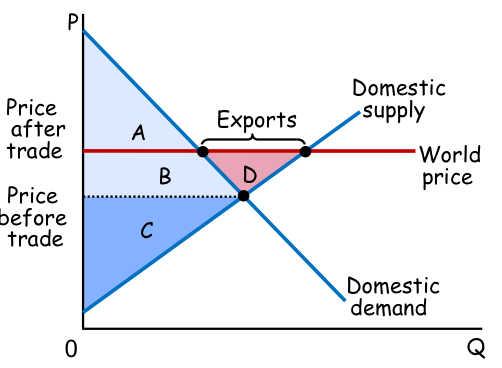
\includegraphics[height=3in]{images/exportCountry.png}
		\caption{Exporting country}
		\label{fig:images_exportCountry}
	\end{figure}
	
\begin{itemize}
	\item Area $D$ shows the increase in total surplus and represents the gain from trade
	\item Domestic producers of the good are better off, and domestic consumers of the good are worse off
\end{itemize}
	
% subsection exporting_country (end)

\subsection{Importing Country} % (fold)
\label{sub:importing_country}
\begin{figure}[htbp]
	\centering
		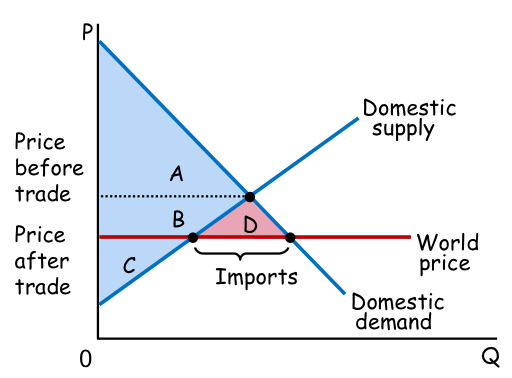
\includegraphics[height=3in]{images/importCountry.png}
	\caption{Importing Country}
	\label{fig:images_importCountry}
\end{figure}

\begin{itemize}
	\item Area $D$ shows the increase in total surplus and represents the gain from trade
	\item Domestic consumers of the good are better off, and domestic producers of the good are worse off
\end{itemize}

% subsection importing_country (end)

\subsection{Trade Policies} % (fold)
\label{sub:trade_policies}

\paragraph{Tariff} % (fold)
\label{par:tariff} 
is a tax on goods produced abroad and sol domestically $\Rightarrow$ Tariffs raise the price of imported goods above the world price by the amount of the tariff (swiss farmers, milk producers). Note the area $D$ and $F$ are deadweight losses. 
\begin{figure}[htbp]
	\centering
		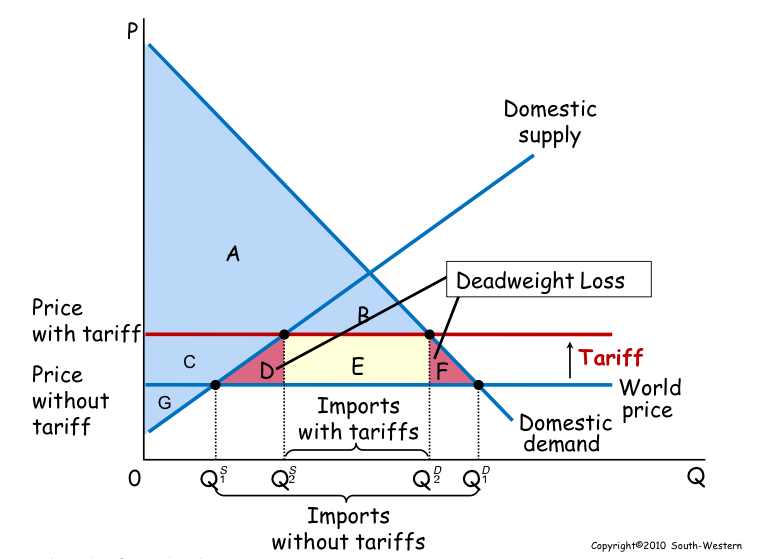
\includegraphics[height=3in]{images/tariff.png}
	\caption{Tariff}
	\label{fig:images_tariff}
\end{figure}

% paragraph tariff (end)
\paragraph{Import Quota} % (fold)
\label{par:import_quota}
 limit on the quantity of a good that can be 
produced abroad and sold domestically.
% paragraph import_quota (end)
\begin{figure}[htbp]
	\centering
		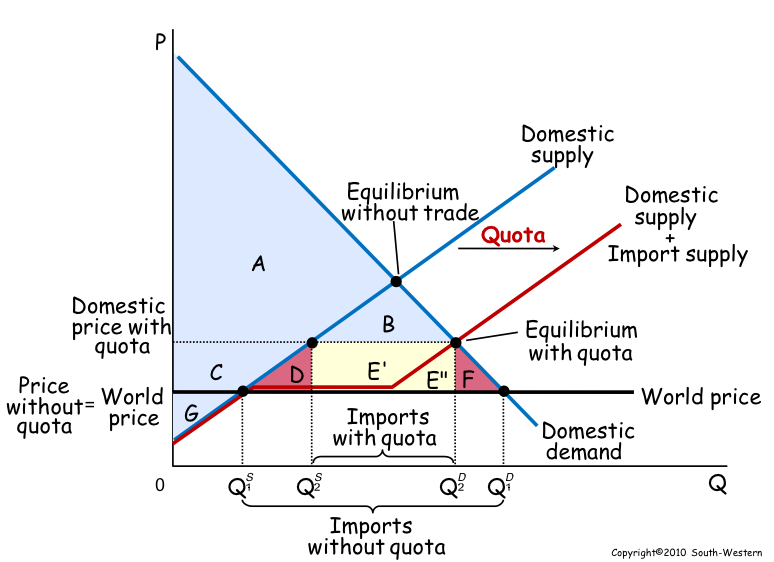
\includegraphics[height=3in]{images/importquota.png}
	\caption{Import quota}
	\label{fig:images_importquota}
\end{figure}

% subsection trade_policies (end)

\subsection{Arguments for restricting Trade} % (fold)
\label{sub:arguments_for_restricting_trade}
\begin{itemize}
	\item Jobs
	\item National Security
	\item Infant Industry
	\item Unfair Competition
	\item Protection as a bargaining Chip
\end{itemize}
% subsection arguments_for_restricting_trade (end)

\subsection{Trade Agreements and The WTO} % (fold)
\label{sub:trade_agreements_and_the_wto}
\paragraph{Unilateral} % (fold)
\label{par:unilateral}
when a country removes its trade restrictions on its own
% paragraph unilateral (end)

\paragraph{Multilateral} % (fold)
\label{par:multilateral}
a country reduced its trade restrictions while other countries do the same.
% paragraph multilateral (end)

% subsection trade_agreements_and_the_wto (end)

\section{Market Failure \& Common Resources}

todo

\section{Public Sector and the tax System}
\subsection{Government spendings} % (fold)
\label{sub:government_spendings}

\paragraph{Government spending} % (fold)
\label{par:government_spending}
includes all transfer payments, the purchase of public goods and services and general public policy program.

Can be measured as $\%$of GDP.
% paragraph government_spending (end)


\subparagraph{Transfer payments} % (fold)
\label{par:transfer_payments}
are government payments not made in exchange for a good or a service, e.g. pensions or unemployment benefits.
% paragraph transfer_payments (end)

% subsection government_spendings (end)


\subsection{Sources of Government Revenues} % (fold)
\label{sub:sources_of_government_revenues}
\paragraph{Public revenues} % (fold)
\label{par:public_revenues}
are defined as tghe sum of financial resources accruing the public sector in order to finance \textbf{national expenditure} and th \textbf{subsidies for the economy}. It comes from
\begin{enumerate}
	\item sales and leasing of goods and ervices
	\item Taxes ad fees
	\item Loans
\end{enumerate}
% paragraph public_revenues (end)
% subsection sources_of_government_revenues (end)


\paragraph{Average tax rate} % (fold)
\label{par:average_tax_rate}
is total tax paid divided by total income.	
% paragraph average_tax_rate (end)

\paragraph{Marginal tax rate} % (fold)
\label{par:marginal_tax_rate}
is the extra tax paid on an additonal pound of income.
% paragraph marginal_tax_rate (end)


\paragraph{Lump-sum Tax} % (fold)
\label{par:lump_sum_tax}
is a tax that is the same amount for every person, regardless of earnings or any actions that the person might take
% paragraph lump_sum_tax (end)

\paragraph{Budget deficit} % (fold)
\label{par:budget_deficit}
When government spends more than it has
% paragraph budget_deficit (end)

\paragraph{National debt} % (fold)
\label{par:national_debt}
is the value of accumulated net borrowing by that state and other public authorities from the economic system and foreign countries.
% paragraph national_debt (end)


\paragraph{Financing of public deficit} % (fold)
\label{par:financing_of_public_deficit}		
can be done in a \textbf{monetary way} (printing banknotes $\rightarrow$ inflation) or in a \textbf{non-monetary} way (issuing fixed-income bonds)

% paragraph financing_of_public_deficit (end)


\subsection{Taxes and efficiency} % (fold)
\label{sub:taxes_and_efficiency}
\paragraph{Efficient tax system} % (fold)
\label{par:efficient_tax_system}
tries to minimize the costs to taxprayers and the governments.

Costs are	\begin{itemize}
	\item tax payment itself
	\item deadweight loss
	\item Administrative burden
\end{itemize}
% paragraph efficient_tax_system (end)
% subsection taxes_and_efficiency (end)

\subsection{Taxes and Equity} % (fold)
\label{sub:taxes_and_equity}

\paragraph{Equity} % (fold)
\label{par:equity}
How should the burden of taxes be divided among the population
% paragraph equity (end)
% subsection taxes_and_equity (end)

\subparagraph{Benefits principle} % (fold)
\label{subp:benefits_principle}
is the idea people should pay taxes based on the benefits they receive from government services.
(those who use car pay petrol tax)
% subparagraph benefits_principle (end)

\subparagraph{Ability to pay prinicple} % (fold)
\label{subp:ability_to_pay_prinicple}
is the idea that tax should be levied on a person according to how well that person can shoulder the burden.

\begin{itemize}
	\item \textbf{Vertical Equity}	taxpayers with greater ability to pay taxes pay more
	\begin{itemize}
		\item Proportional tax
		\item Regressive tax
		\item Degressive tax
	\end{itemize}
	\item \textbf{Horizontal equity} idea that taxpayers with same ability to pay taxes pay the same amount.
\end{itemize}
% subparagraph ability_to_pay_prinicple (end)

\subsection{Tax Incidence and Tax Equity} % (fold)
\label{sub:tax_incidence_and_tax_equity}

Tax equity and efficiency are the two most important goals of the tax system.

\paragraph{Tax incidence} % (fold)
\label{par:tax_incidence}
is the study of who shares the burden of the tax
% paragraph tax_incidence (end)

% subsection tax_incidence_and_tax_equity (end)

\section{The Cost Of Production}

\subsection{Introduction} % (fold)
\label{sub:introduction}
Behind the supply curve
\begin{itemize}
	\item Production function
	\item Cost function
\end{itemize}
% subsection introduction (end)

\subsection{Production theory} % (fold)
\label{sub:production_theory}
\paragraph{Production Technology} % (fold)
\label{par:production_technology}
Combination of inputs in order to produce finished goods and services
% paragraph production_technology (end)
% subsection production_theory (end)

\paragraph{Cobb Douglas Production Function} % (fold)
\label{par:cobb_douglas_production_function}
\begin{equation}
	Q = zC^{\alpha}L^{\beta}
\end{equation}
if CRS, constant return to scale, (see system dynamics), $\alpha+\beta=1$, IRS and DRS also exist
% paragraph cobb_douglas_production_function (end)


\subsection{Costs} % (fold)
\label{par:costs}

\begin{equation}
	\text{Profit} = \text{Total revenue} - \text{Total cost}
\end{equation}
% paragraph costs (end)

\paragraph{Economic profit} % (fold)
\label{par:economic_profit} the total revenue minus total cost, including both explicit and implicit costs.

\paragraph{Accounting profit} % (fold)
\label{par:accounting_profit}
total revenue - total explicit cost
% paragraph accounting_profit (end)

% paragraph economic_profit (end)

\paragraph{Production Function} % (fold)
\label{par:production_function}
reltionship between quantity of inputs used and the quantity of output 
% paragraph production_function (end)

\paragraph{Marginal product} % (fold)
\label{par:marginal_product}
Increase in output that arise from an additional unit of input

% paragraph marginal_product (end)

\paragraph{Diminishing marginal product} % (fold)
\label{par:diminishing_marginal_product}
When the derivative of the marginal product is negative, the double derivtaive of the production function is negative...

% paragraph diminishing_marginal_product (end)

\paragraph{Fixed Costs $FC$} % (fold)
\label{par:fixed_costs}
Costs that do not vary with the quantity of output produced
% paragraph fixed_costs (end)

\paragraph{Variable costs $VC$} % (fold)
\label{par:variable_costs}
Costs that DO vary with amount of output produced
% paragraph variable_costs (end)

\paragraph{Total Costs $TC$} % (fold)
\label{par:total_costs_tc_}
\begin{equation}
	TC = FC + VC +\dots
\end{equation}
% paragraph total_costs_tc_ (end)

\paragraph{Average Total Cost $AVC$} % (fold)
\label{par:average_total_cost}
\begin{equation}
	AVC = \frac{VC}{Q}
\end{equation}
The curve is usually U-shaped
% paragraph average_total_cost (end)

\paragraph{Marginal cost $MC$} % (fold)
\label{par:marginal_cost}
\begin{equation}
	MC = \frac{dTC}{dQ}
\end{equation}
% paragraph marginal_cost (end)

\paragraph{Efficient scale} % (fold)
\label{par:efficient_scale}
quantity of output that minimizes average total cost
% paragraph efficient_scale (end)


\subsection{Costs in the short and long run}
in the short run, some costs are fixed, in the long run, fixed become variable costs.

\subsection{Economies and diseconomies of scale}
\begin{figure}[htbp]
	\centering
		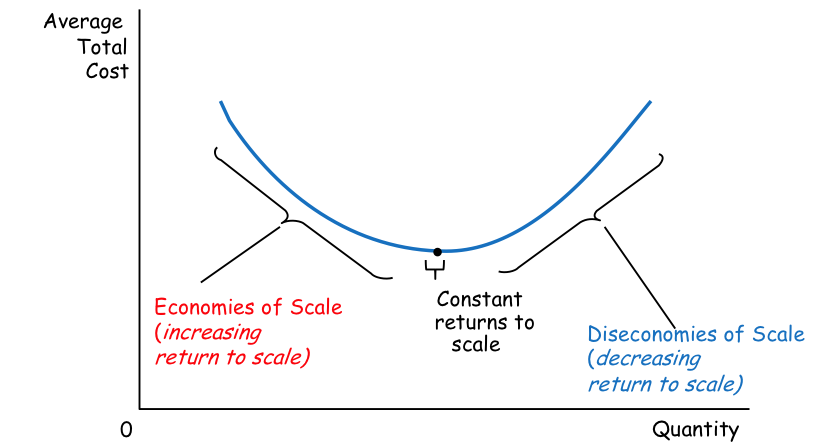
\includegraphics[height=3in]{images/ecoscale.png}
	\caption{Economy of scale}
	\label{fig:images_ecoscale}
\end{figure}

\paragraph{Economies of Scope} % (fold)
\label{par:economies_of_scope}
If the joint output of a single firm is greater than 
the output that could be achieved by two different 
firms when each produces a single product, we speak 
of economies of scope.
% paragraph economies_of_scope (end)

\paragraph{Learning Curve} % (fold)
\label{par:learning_curve}
A firm‘s production cost may fall over time as managers and workers 
become more experienced and more effective at using the available 
plant and equipment. The learning curve shows the extent to which 
hours of labor needed per unit of output fall as the cumulative output 
increases. 

% paragraph learning_curve (end)


%hapter 14
\section{Firms in Competitive Markets}
\paragraph{Competitive Market} % (fold)
\label{par:competitive_market}
a market with many buyers and sellers that are \emph{price takers}		
% paragraph competitive_market (end)

\paragraph{Average revenue} % (fold)
\label{par:average_revenue}
\begin{equation}
	AR = \frac{TR}{Q}
\end{equation}
where $TR=P\cdot Q$ is the total revenue and $Q$ the quantity sold.
% paragraph average_revenue (end)

\paragraph{Marginal revenue} % (fold)
\label{par:marginal_revenue}
\begin{equation}
	MR = \frac{\operatorname{d}TR}{\operatorname{d}Q}
\end{equation}
For a competitive firm the following holds
\begin{equation}
	P = AR = MR
\end{equation}

% paragraph marginal_revenue (end)


\paragraph{Profit maximization} % (fold)
\label{par:profit_maximization}
a firm maximizes its profit when the "marginal profit" is zero, that is
\begin{equation}
	\text{"marginal profit"}
	=\frac{\operatorname{d}(TR-TC)}{dQ}
	=\frac{dTR}{dQ}-\frac{dTC}{dQ}=0
\end{equation}

\paragraph{Firm's decision to shutdown} % (fold)
\label{par:firm_s_decision_to_shutdown}
\begin{eqnarray*}
	\text{shutdown if }&
	TR < VC\nonumber\\
&	TR/Q < VC/Q\nonumber\\
	&P < AVC
\end{eqnarray*}
% paragraph firm_s_decision_to_shutdown (end)
% paragraph profit_maximization (end)

\paragraph{Firm 's decision  to quit in the long run} % (fold)
\label{par:firm_s_decision_to_quit_in_the_long_run}
\begin{eqnarray*}
		\text{exit if }&
		TR < TC\nonumber\\
	&	TR/Q < TC/Q\nonumber\\
		&P < ATC
\end{eqnarray*}

reciprocally	
\begin{eqnarray*}
		\text{enter if }
		&P > ATC
\end{eqnarray*}

% paragraph firm_s_decision_to_quit_in_the_long_run (end)

\subparagraph{Sunk cost} % (fold)
\label{subp:sunk_cost}

a cost that has already been committed and cannot be recovered
% subsection sunk_cost (end)par

\paragraph{Measuring profit for the competitive firms} % (fold)
\label{par:measuring_profit_for_the_competitive_firms}
\begin{eqnarray*}
	\text{Profit} &=& TR -TC\nonumber\\
	&=& (TR/Q -TC/Q)\cdot Q\nonumber\\
	&=& (P-ATC)\cdot Q
\end{eqnarray*}

%todo: put figure 14.5 in here

% paragraph measuring_profit_for_the_competitive_firms (end)

\paragraph{Zero Profit} % (fold)
\label{par:zero_profit}
In the long runy, competitive firms make a zero profit. (however this is \underline{not} an accountant profit, it includes implicit costs)
% paragraph zero_profit (end)


%%% 10.12.10 

\section{Monopoly}
A firm that is the sole seller of a product without close substitutes


\section{Monopolistic Competition}
%course of december 17


\subsection{Monopolistic Competitions} % (fold)
\label{sub:monopolistic_competitions}
a market structure in which many firms sell products that are similar but not identical.


% subsection monopolistic_competitions (end)

\subsection{Monopolisitic Competition in the Short Run} % (fold)
\label{sub:monopolisitic_competition_in_the_short_run}

% subsection monopolisitic_competition_in_the_short_run (end)

\subsection{Monopolistic Competition in the Long Run} % (fold)
\label{sub:monopolistic_competition_in_the_long_rub}
Monopolistic competition is one of the four market structure. Examples: gasoline, cars.

Attributes
\begin{itemize}
	\item many sellers
	\item product differentiation
	\item free entry and exit
\end{itemize}

In the short run a monopoly market and monopolistic competitive market are identical (choose quantity as well as price).

\begin{itemize}
	\item Short run economic profit encourage new firms to enter the market
	\item Short run economic loss encourage firms to exit the market
\end{itemize}

Firms will enter and exit the market until firms are making zero profit.

Two characterstics
\begin{itemize}
	\item As in a \textbf{monopoly}, price exceeds marginal cost
	\item As in a \textbf{competitive market}, price equals average total cost
\end{itemize}
\begin{figure}[htbp]
	\centering
		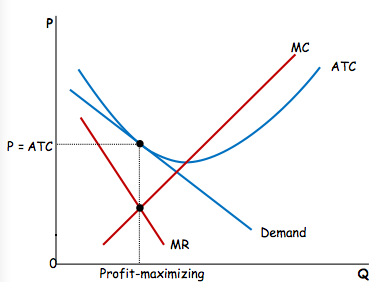
\includegraphics[height=3in]{images/lrmonocom.png}
	\caption{Monopolistic Competition in the Long Run}
	\label{fig:images_lrmonocom}
\end{figure}



% subsection monopolistic_competition_in_the_long_rub (end)

\subsection{Comparison of different Market Structures} % (fold)
\label{sub:comparison_of_different_market_structures}
\begin{figure}[htbp]
	\centering
		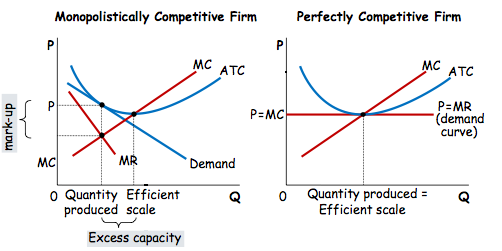
\includegraphics[height=3in]{images/comptmonovsperfect.png}
	\caption{Monopolistic vs perfect competition}
	\label{fig:images_comptmonovsperfect}
\end{figure}

\subsubsection{Mark up over original cost}
\begin{itemize}
	\item for a competitive firm marginal cost equals price
	\item for a monopolisticalls competitive firm, price exceeds marginal cost
	\item because price exceed marginal cost, an extra unit sold at the posted price means more profit for the monopolistically competitive firm
\end{itemize}

\subsubsection{Excess capacity}
\begin{itemize}
	\item Free entry results in competitive firms producing at the point where average total cost is minimized, which is the efficient scale of the firm.
	\item In monopolistic competition, output is less than the efficient scale of perfect competition.
\end{itemize}
	
% subsection comparison_of_different_market_structures (end)

\subsection{Monopolistic Competition and Welfare} % (fold)
\label{sub:monopolistic_competition_and_welfare}
Monopolistic does not have all the desirable properties of perfect competition.
\begin{itemize}
	\item Normal deadweight loss, caused by mark-up of price over marginal cost
	\item Number of firms is not "ideal"
\end{itemize}

... but the administrative burden of regulating the different would be overwhelming.
	
% subsection monopolistic_competition_and_welfare (end)

\subsection{Advertising} % (fold)
\label{sub:advertising}
When firms sell differentiated products and charge prices above marginal cost, each firm has an incentive to advertise in order to attract more buyers. Typically between 10 and 20\% of revenue.
% subsection advertising (end)

\subsection{Brand Names}
\begin{itemize}
	\item $-$ consumers perceive changes that do not exist
	\item $+$ ensure consumers buy a product of high quality
\end{itemize}

\subsection{Introduction to Oligopoly and Game theory} % (fold)
\label{sub:models_of_imperfect_competitions}
\subsubsection{Game theory}
\paragraph{Dominance} % (fold)
\label{par:dominance}
A strategy is dominant if it outperforms all other choices no matter what opposing players do.

\paragraph{Rationalizable strategies} % (fold)
\label{par:rationalizable_strategies}
are the sets of all strategies that are not strictly dominated.
% paragraph rationalizable_strategies (end)
% paragraph dominance (end)
% subsection models_of_imperfect_competitions (end)


\subsection{Monopoly and its Causes} % (fold)
\label{sub:monopoly_and_its_causes}

% subsection monopoly_and_its_causes (end)

\paragraph{Why Monopolies Arise} % (fold)
\label{par:why_monopolies_arise}
There are generally three causes
\begin{itemize}
	\item A key resource is owned by a single firm
	\item Government created monopolies: patent and copyright
	\item Natural monopoly: a monopoly that arises because a single firm can supply a good or service to an entire market at a smaller cost than could two or more firms.
\end{itemize}
% paragraph why_monopolies_arise (end)


\paragraph{Price Discrimination} % (fold)
\label{par:price_discrimination}
the business practice of selling the same good at two different prices.
% paragraph price_discrimination (end)





\section{Oligopoly}



\end{document}
